\documentclass[12pt, a4paper, oneside]{ctexart}
\usepackage{amsmath,amsthm,amssymb,graphicx}
\usepackage{float}
\usepackage{hyperref}
%author:潘宇琦


\begin{document}
我在更新这个网站的时候，突然想到刚上大二的同学可能没有使用latex的经验，但是latex确确实实是近到实验报告远到读研都必须掌握的技能，甚至有学院老师直言会latex是一个较好的加分项，所以我决定写一篇latex教程，基本覆盖一些本科阶段的latex使用场景，帮助大家快速上手。

首先，latex是什么？

与我们之前就耳熟能详的Word类似，latex也是一种文档排版系统，大家或多或少都使用过Word，Word界面有各种各样的按钮、图标，点击这些按钮就可以实现不同的功能，比如说文字的加粗或者调整行间距等等，但是latex并没有这些按钮，latex排版是通过一系列命令来对文字进行操作，听上去很困难，但是实际上latex的命令是非常容易上手的，而且你需要掌握的命令的数量非常非常少，掌握这些最基本的，就足够排版出相当规范的文档。我们前面提到过latex是读研必备的技能，是因为latex对于数学公式的排版效果要远超Word，这也是这个网站的源文件格式都采用.tex的原因。

OK，那我们应该如何使用latex呢？

使用方法有两类，一类是使用在线编辑器，直接在浏览器中搜索就可以找到很多，打开然后在线编辑就能得到你想要的，但是我个人并不推荐，在线编辑器的功能不是很全面，而且必须联网使用，我个人觉得使用体验一般，另一类是使用本地编辑器，安装在自己的电脑上，离线使用，我个人非常非常推荐这种方式。

我把安装过程分为两部分，第一部分是texlive的安装，第二部分是TexStudio的安装，前者是latex的核心，后者是一个编辑器，我需要提醒的是，一定一定要先完成第一部分的安装，再进行第二部分的安装，请不要混乱顺序！！

首先我们要安装texlive，因为我们前面提到过latex是基于命令，也就是代码的排版系统，所以其运行需要latex环境，也就是这里的texlive，这里面包含了latex运行所需要的命令和包，也是为什么我们要先安装它。

首先我们打开\url{https://mirrors.tuna.tsinghua.edu.cn/CTAN/systems/texlive/Images/}，这是清华大学的开源软件镜像站，我们找到texlive.iso，如下图所示，单击下载，下载速度依网速而定。

\begin{figure}[H]
	\centering
	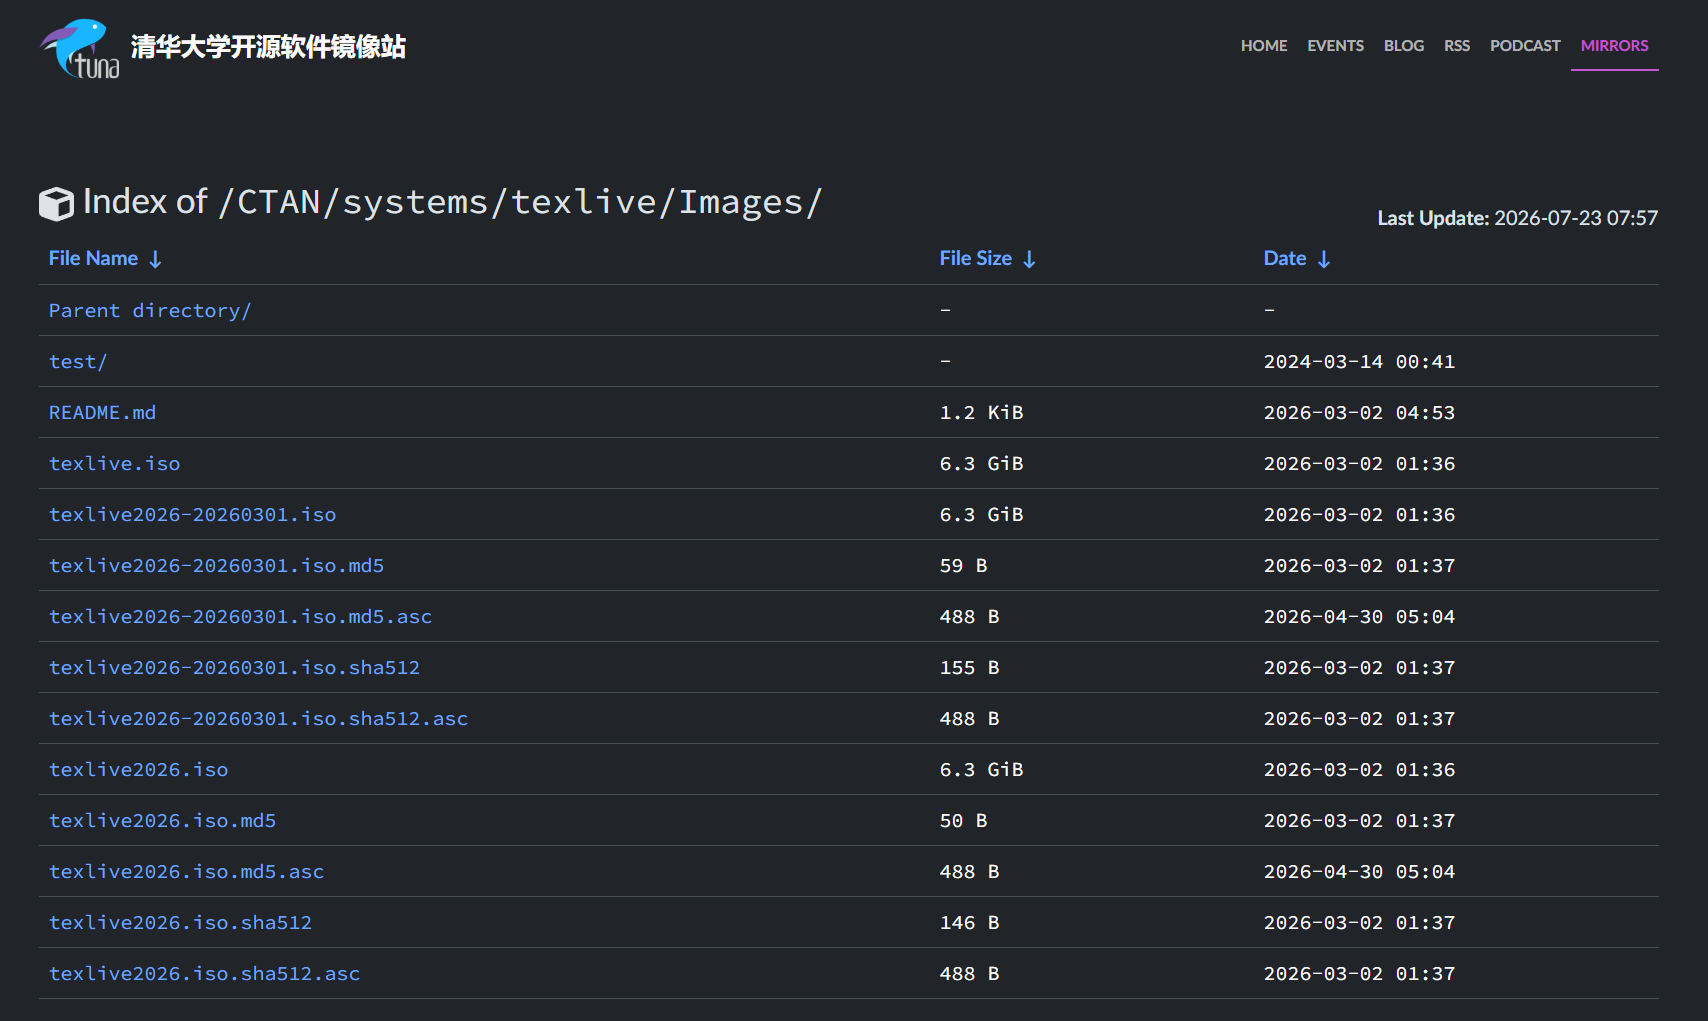
\includegraphics[scale=0.35]{figure/00/1.png}
	\caption{Ubuntu20.04安装成功}
\end{figure}


\end{document}










